% Manuscript for BMC Medical Imaging (Research article).
% Structure follows the BMC Medical Imaging submission guidelines: title page, structured abstract (<= 350 words),
% keywords, Background, Methods, Results, Discussion, Conclusions, Abbreviations, Declarations, References (Vancouver).
% Numbers: paper/ (generated tables) and docs/REPLICATION_RESULTS.md (final, 2026-11-21).
\documentclass[12pt]{article}
\usepackage[a4paper,margin=2.5cm]{geometry}
\usepackage[T1]{fontenc}
\usepackage{lmodern,amsmath,amssymb,booktabs,graphicx,array,setspace,xcolor}
\usepackage[numbers,sort&compress]{natbib}
\usepackage[hidelinks]{hyperref}
\usepackage{lineno}
\linenumbers
\doublespacing
\setlength{\emergencystretch}{2em}

\begin{document}

\begin{center}
{\Large\bfseries Masking cannot remove what is inside the region of interest: location-dependent shortcut learning
in medical image classification, validated against published methods}\par\bigskip
Hossam Elkady$^{1,*}$\par\medskip
{\small $^1$[Department, University, City, Country]\\
$^*$Corresponding author: [email address]}
\end{center}

\section*{Abstract}
\paragraph{Background} Medical image classifiers exploit acquisition artifacts such as hair, sonographer calipers and
intestinal debris that correlate with the diagnosis. The standard defence restricts the classifier to the region of
interest (ROI) by masking or by penalising evidence outside a segmentation. We asked whether this defence depends on
where the artifact lies relative to the ROI, and what to use when it lies inside.

\paragraph{Methods} We built pre-registered traps from real artifacts in four diseases and three modalities
(dermoscopy, thyroid and ovarian ultrasound, capsule endoscopy), trained with the artifact on 90\% of positive and 10\%
of negative images and tested with the association reversed. We transplanted the same real artifacts inside or outside
the ROI of the same images, proposed a class-conditional mean constraint on masked frozen features, and validated it
against eight published mitigation papers in their own and in our environments under registered rules.

\paragraph{Results} Masking removed out-of-ROI shortcuts but left in-ROI ones largely intact: the location crossover in
reversed-test AUROC was $+0.15$ to $+0.38$ across cohorts, and transplanting the same artifact across the ROI boundary
reproduced it ($+0.07$ to $+0.50$). On real thyroid calipers inside the nodule, the constraint beat two published
methods in all four registered comparisons (frozen DINOv2: 0.716 vs ISNet 0.561 and RR-ClArC 0.467), with higher
clean AUROC. On published dermoscopy trap sets it beat EPVT at both bias levels ($+0.086$ and $+0.031$ AUROC) and
exceeded DISC run from its official code (0.736 vs 0.489). ISNet, a mask-based method, ignored class marks outside the
lungs but relied on them entirely once they were moved inside. The constraint was not better than a
segmentation-supervised method (tie) and did not remove class-specific marks inside the ROI or an invisible
whole-image trigger. Five of eight published results did not reproduce from the authors' code.

\paragraph{Conclusions} ROI masking protects against artifacts only outside the ROI. Where artifacts may lie inside it
and image-level artifact labels exist, a class-conditional constraint on masked frozen features should be used, and
audits of masked models should report artifact location and performance on shortcut-conflicting cases.

\paragraph{Keywords} Shortcut learning; Spurious correlation; Region of interest; Masking; Artifacts; Dermoscopy;
Ultrasound; Capsule endoscopy; Reproducibility

\clearpage
\section*{Background}
Deep classifiers for medical images often rely on features that correlate with the label in the training data but are
not evidence of disease \cite{geirhos2020shortcut,degrave2021ai}. Surgical skin markings \cite{winkler2019markings} and
ruler scale bars \cite{winkler2021scalebars} changed the melanoma predictions of a market-approved dermoscopy system,
and pneumothorax classifiers detect the chest drain that treats the condition
\cite{oakden2020hidden,rueckel2021pneumothorax,jimenez2023shortcuts}. Such correlations arise from clinical practice
itself (suspicious lesions are measured and marked), so they are present in every retrospectively collected dataset.

The most widely recommended defence restricts the classifier to the region of interest (ROI): the lesion is segmented
and the rest discarded, or relevance outside the segmentation is penalised \cite{maron2021confounding,bassi2024isnet}.
This assumes that the shortcut lives in the background. Rulers, hair, calipers and debris often lie on the lesion. Several
studies note this risk without testing it \cite{maron2021confounding,viviano2021saliency,benahmed2022multisite,pahde2025ensuring},
and synthetic studies varied the distance of a bias from the disease region, but always outside it
\cite{stanley2023framework,stanley2024simba}. Benchmarks of shortcut mitigation in medical imaging mostly use global
attributes such as patient sex or hospital \cite{mueller2026shortcut,viviano2021saliency}, which have no location.

We test whether ROI restriction depends on the location of a real artifact relative to the ROI, explain why, propose a
remedy, and validate it against published methods in their own and in our test designs.

\section*{Methods}
\subsection*{Data}
\emph{Dermoscopy:} ISIC 2019 (25,331 images) with hair masks and lesion masks (manual for HAM10000, otherwise from a
U-Net trained on ISIC 2018 Task 1); ISIC 2020 (32,997 images of 2,056 patients) as new patients. \emph{Thyroid
ultrasound:} TN3K \cite{gong2021tn3k} (3,493 images, 1,210 malignant, biopsy-confirmed; patient-disjoint official split)
with manual nodule masks and calipers segmented by a frozen rule-based detector. \emph{Ovarian ultrasound:} MMOTU
\cite{zhao2022mmotu} (1,202 images). \emph{Capsule endoscopy:} SEE-AI \cite{seeai2023} erosion and polyp-like frames, with
debris, bubbles and bile segmented by a linear probe on DINOv2 patch tokens. Splits were grouped by lesion or patient
identifier where available and otherwise by perceptual hash.

\subsection*{Trap design}
Let $Y$ be the diagnosis and $A$ the presence of an artifact. A trap trains with $P(A{=}1\mid Y{=}1)=0.9$ and
$P(A{=}1\mid Y{=}0)=0.1$ and tests on a correlated environment (same rates), a reversed environment (rates swapped) and
a clean environment (artifact independent of the label), following earlier reversed-test designs
\cite{arjovsky2019irm,bissoto2020debiasing,puli2022nurd,viviano2021saliency,bassi2024isnet}. Trap~A uses images whose
real artifact overlaps the ROI ($r\ge0.5$, with $r$ the fraction of the artifact inside the ROI), Trap~B images whose
artifact lies outside it ($r<0.1$); both share one artifact-free group. The real-artifact transplant pastes one real
artifact instance inside ($r\ge0.95$) or outside ($r=0$) the ROI of the same artifact-free images, with neutral tissue
pasted through the same mask as a paste-edge control. The primary metric is reversed-test AUROC; the \emph{location
crossover} $[\text{mask}-\text{ERM}]_{\text{out}}-[\text{mask}-\text{ERM}]_{\text{in}}$ summarises each design
(Fig.~\ref{fig:design}).

\begin{figure}[t]\centering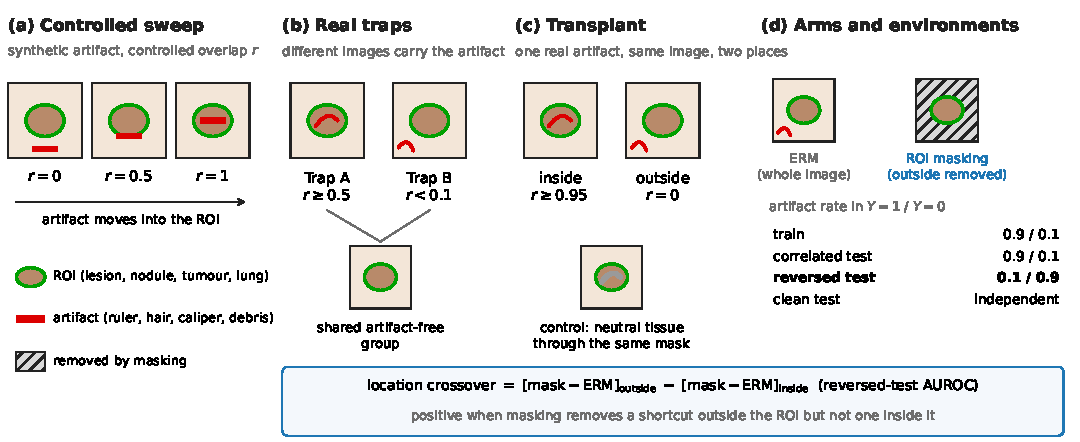
\includegraphics[width=\linewidth]{../paper/figures/design.pdf}
\caption{Study design. (a) Controlled sweeps paste a synthetic artifact at a controlled overlap $r$ with the ROI.
(b) Real traps compare images whose real artifact lies inside (Trap~A) or outside (Trap~B) the ROI. (c) The transplant
pastes one real artifact inside or outside the ROI of the same images, with neutral tissue as a paste-edge control.
(d) ERM sees the whole image; ROI masking removes everything outside the ROI.}\label{fig:design}\end{figure}

\subsection*{Models and the class-conditional constraint}
Unless stated otherwise, backbones were frozen (DINOv2 ViT-B/14 and others) and linear heads were fitted; regularisation
and thresholds were chosen on clean validation data only. The \emph{class-conditional constraint} uses the image-level
artifact label $a$ during training only. With $x$ the frozen features of the masked image, we compute the within-class
mean differences $\delta_y=\mu(x\mid a{=}1,y)-\mu(x\mid a{=}0,y)$, project the features onto the orthogonal complement
of $\delta_0,\delta_1$ (or of their average; chosen on validation data) and fit a logistic head on all training images.
Within each class the head cannot score images with and without the artifact differently on average, and no image is
down-weighted. It is the first-moment linear case of counterfactual invariance \cite{veitch2021counterfactual,makar2022causally},
related to class artifact compensation \cite{anders2022clever,pahde2025ensuring}, but removes within-class differences,
is applied after masking, and needs only the masked image at test time.

\subsection*{Validation against published methods}
We selected published mitigation papers on medical image classification with released code, public data, a localized
artifact that varies within each class, and a published robustness number. For each paper we ran its best method with the
authors' code (reproduction gate: within 0.05 of the published value in the paper's metric; this tolerance was widened
from 0.03 for every paper after the first gate results, a deviation we report). If the gate passed (tier~1), our method
counted as having beaten theirs only if the 95\% CI of the paired difference, Holm-adjusted, lay above zero; otherwise
(tier~2) we compared with our run of the official code under identical conditions and made no claim against the
published number. Four variants were registered: (a) the constraint on the competitor's own features; (b) on frozen
DINOv2 features of masked images; (c) the label-free U-MtE; (d) on an EfficientNet-B0 (5.3\,M parameters) trained on masked
images. In our environment (thyroid calipers, three folds), ISNet \cite{bassi2024isnet} and RR-ClArC \cite{pahde2025ensuring}
were trained with their published recipes under one registered selection rule.

\subsection*{Statistics and registration}
Uncertainty is a paired crossed bootstrap: training seeds or folds are resampled as clusters, and each test image
receives one Poisson weight shared across clusters (10,000 replicates). Each family of tests is Holm-corrected. Every
confirmatory analysis was registered in a document committed before its results; analyses decided after their data
were seen are labelled exploratory.

\section*{Results}
\subsection*{Masking fails when the artifact is inside the ROI}
In real traps, masking removed out-of-ROI shortcuts but left in-ROI ones largely intact: the location crossover was
$+0.147$ (hair), $+0.239$ (thyroid), $+0.170$ (ovary) and $+0.377$ (capsule), all Holm-significant
(Table~\ref{tab:law}). Propensity-matched traps gave the same result, and transplanting the same real artifact across the
ROI boundary of the same images reproduced it (hair $+0.25$, thyroid $+0.28$, ovary $+0.07$, capsule $+0.50$), beyond
the paste-edge control in hair and thyroid. The effect held for five masking implementations, fell continuously with
the artifact--ROI overlap, replicated across encoders, end-to-end fine-tuning and new patients, and a two-parameter
linear-Gaussian account predicted 84 registered results with mean absolute error 0.011 AUROC. On unaltered clinical
data masking barely changed overall AUROC, but lowered it on shortcut-conflicting cases and new patients.

\begin{table}[t]\centering\small
\caption{Location crossover (reversed-test AUROC, DINOv2; 95\% crossed CIs). Real traps compare different artifact-bearing
images; the transplant pastes one real artifact inside or outside the ROI of the same images.}\label{tab:law}
\begin{tabular}{lccc}\toprule
Cohort & Real traps & Matched traps & Transplant\\\midrule
Dermoscopy hair & $+0.147$ [$+0.109, +0.185$] & $+0.154$ [$+0.122, +0.187$] & $+0.253$ [$+0.214, +0.293$]\\
Thyroid calipers & $+0.239$ [$+0.196, +0.280$] & $+0.238$ [$+0.186, +0.291$] & $+0.277$ [$+0.256, +0.298$]\\
Ovarian calipers & $+0.170$ [$+0.087, +0.253$] & $+0.163$ [$+0.049, +0.274$] & $+0.074$ [$+0.044, +0.104$]\\
Capsule debris & $+0.377$ [$+0.326, +0.425$] & infeasible & $+0.497$ [$+0.427, +0.567$]\\
\bottomrule\end{tabular}\end{table}

\subsection*{The class-conditional constraint}
Against a registered criterion for dominating masking (42 components), the constraint was better than masking in every
Trap~A, by $+0.118$ (held-out ovary) to $+0.330$ (thyroid, 0.400 to 0.730), and on every set of conflicting cases. It met
40 of 42 components; it failed non-inferiority on the thyroid split (inconclusive, $-0.002$ [$-0.011, +0.007$]) and on
ISIC 2020 overall ($-0.021$ [$-0.027, -0.016$]).

\subsection*{Validation against published methods}
Table~\ref{tab:repl} summarises the eight papers. \emph{In our environment}, with calipers inside the nodule, both
registered variants of the constraint beat ISNet and RR-ClArC in all four comparisons and had higher clean AUROC
(Table~\ref{tab:phase5}); ISNet was better with calipers outside the nodule (0.673) than inside it (0.561), as the
location account predicts for a method that acts only outside the ROI. \emph{In their environments}, EPVT
\cite{yan2023epvt,yan2025pldg} reproduced (five seeds) and the constraint on frozen DINOv2 features beat it at both bias
levels of the dermoscopy trap sets \cite{bissoto2022artifact} (0.782 vs 0.696 and 0.806 vs 0.775); applied to EPVT's own
features the constraint also improved on EPVT. On artifact-free images, this variant was 0.02--0.04 AUROC below EPVT,
while the trained EfficientNet-B0 variant was within 0.01. DISC \cite{wu2023disc} did not reproduce; its released code
shares one image cache across trap sets, and our runs with this misalignment matched the published baseline. Under
identical conditions all four variants exceeded DISC from its official code (0.736 vs 0.489, $+0.247$ [$+0.204, +0.290$])
and the published DISC (0.551) and CBDebug \cite{enouen2026cbdebug} (0.580) values. In ISNet's pipeline, moving its
class marks from the image corner into the lungs changed ISNet from ignoring them (macro-F1 0.84/0.83/0.83 with
own-class, no and swapped marks) to relying on them alone (0.998/0.167/0.000).

\begin{table}[t]\centering\small
\caption{Thyroid calipers inside the nodule (Trap~A), registered confirmatory comparison. Reversed-test AUROC, mean
$\pm$ SD over three folds; $\Delta$ with 95\% CI, Holm over four.}\label{tab:phase5}
\begin{tabular}{lccc}\toprule
Method & Trap A (inside) & Trap B (outside) & Clean\\\midrule
Constraint, frozen DINOv2 & \textbf{0.716} $\pm$ 0.027 & 0.789 & 0.797\\
Constraint, EfficientNet-B0 & 0.690 $\pm$ 0.076 & 0.746 & 0.733\\
ISNet \cite{bassi2024isnet} & 0.561 $\pm$ 0.172 & 0.673 & 0.633\\
RR-ClArC \cite{pahde2025ensuring} & 0.467 $\pm$ 0.049 & 0.595 & 0.643\\
ERM & 0.440 & 0.546 & 0.625\\\midrule
\multicolumn{4}{l}{DINOv2 vs ISNet $+0.155$ [$+0.019, +0.316$]; vs RR-ClArC $+0.249$ [$+0.192, +0.304$]}\\
\multicolumn{4}{l}{EfficientNet-B0 vs ISNet $+0.129$ [$+0.035, +0.239$]; vs RR-ClArC $+0.224$ [$+0.159, +0.292$]}\\
\bottomrule\end{tabular}\end{table}

\begin{table}[t]\centering\footnotesize
\caption{Validation against eight published papers. Tier~1: reproduced, verdicts apply; tier~2: not reproduced,
descriptive comparison with our run of the official code.}\label{tab:repl}
\begin{tabular}{>{\raggedright\arraybackslash}p{4.1cm}>{\raggedright\arraybackslash}p{2.5cm}>{\raggedright\arraybackslash}p{1.1cm}>{\raggedright\arraybackslash}p{4.3cm}}\toprule
Paper (artifact) & Reproduced & Tier & Result\\\midrule
EPVT, MICCAI 2023 / IEEE TMI 2025 (hair, rulers, gel) & yes (5 seeds) & 1 & beaten at both bias levels\\
RR-ClArC, AAAI 2024 (invisible whole-image trigger) & yes & 1 & not beaten (no location)\\
DISC, ICML 2023 (hair) & no & 2 & all variants above official code\\
RR-ClArC, Mach.\ Learn.\ 2025 (inserted vignette) & no & 2 & above official code and published value\\
ISNet, Nat.\ Commun.\ 2024 (class marks) & no (external test) & 2 & ISNet fails with marks inside the ROI\\
Viviano et al., ICLR 2021 (tube; location test, 3 seeds) & yes & formal & masking's crossover supported; gain over their model not significant\\
Saab et al., MLHC 2022 (trap sets) & no & 2 & tie ($+0.023$ [$-0.029, +0.076$])\\
Reveal to Revise, MICCAI 2023 & no & --- & not compared\\
\bottomrule\end{tabular}\end{table}

\section*{Discussion}
ROI masking is not a neutral preprocessing step: it removes shortcuts that live outside the ROI and retains, or amplifies,
those inside it, because it discards competing evidence while keeping the artifact. The same holds for a published
method that penalises relevance outside the ROI: ISNet worked as designed with marks in the image corner and relied on
them entirely once they were moved into the lungs, and on real calipers it was better when they lay outside the nodule.
The constraint addresses the in-ROI case without needing artifact information at test time, and it beat published
methods both in our test design and in a published one.

\paragraph{Limitations} First, the constraint needs image-level artifact labels during training; the label-free variant
(U-MtE) did not beat the published methods inside the ROI. Second, it removes within-class artifact directions, so it
cannot remove marks whose shape itself identifies the class (ISNet's design) and does not address artifacts without a
location, such as an invisible whole-image trigger. Third, frozen encoders give up some clean accuracy on fine-grained
tasks (0.02--0.04 AUROC against EPVT on artifact-free images); a small trained encoder kept clean accuracy but absorbs
strong shortcuts. Fourth, a segmentation-supervised method, which uses lesion masks as training targets, matched it.
Fifth, the reproduction tolerance was widened after the first gates, EPVT's reproduction margin was smaller than the
uncertainty of reading its published figure, and several published results did not reproduce; we report these
comparisons as descriptive and have contacted the authors. Finally, heads often selected the smallest regularisation
strength of their grid, and most traps use 90/10 schedules rather than naturally occurring prevalence.

\paragraph{Reproducibility of published results} Five of the eight published results did not reproduce from the
authors' code, and for three we identified concrete causes: an image cache shared across trap sets (DISC), a mixup
label pairing that differs from the paper (EPVT) and checkpoint selection (Saab et al.). Reported comparisons in this
area should state whether the comparator was reproduced.

\section*{Conclusions}
Artifact location relative to the ROI decides whether ROI restriction works. Where artifacts may lie inside the ROI and
image-level artifact labels exist, a class-conditional constraint on masked frozen features should be used instead of
masking alone; it outperformed published mitigation methods on real in-ROI calipers and on published dermoscopy trap
sets. Audits of masked models should report artifact location and performance on shortcut-conflicting cases.

\section*{Abbreviations}
AUROC: area under the receiver operating characteristic curve; CI: confidence interval; ERM: empirical risk minimisation;
ROI: region of interest; U-MtE: unsupervised mask-then-erase (label-free variant).

\section*{Declarations}
\paragraph{Ethics approval and consent to participate} Not applicable: the study uses only publicly available, de-identified
datasets (ISIC, TN3K, MMOTU, SEE-AI, NIH ChestX-ray14, PadChest, BrixIA, CheXpert, BIMCV COVID-19+) under their licences.
\paragraph{Consent for publication} Not applicable.
\paragraph{Availability of data and materials} All datasets are public (see Methods). Code, pre-registrations,
per-image predictions and result files are available at [repository URL].
\paragraph{Competing interests} The author declares no competing interests.
\paragraph{Funding} [Funding statement, or ``Not applicable''].
\paragraph{Authors' contributions} H.E. designed the study, ran the experiments, analysed the results and wrote the
manuscript. [Add co-authors and supervisor as appropriate.]
\paragraph{Acknowledgements} [Supervisor and others.]

\bibliographystyle{vancouver}
\bibliography{../paper/refs}
\end{document}
